\section[Photonic RC with frequency multiplexed neurons]{Photonic reservoir computer with wavelength division multiplexed neurons}

\begin{frame}{Working principle}
	\begin{figure}
		\centering
		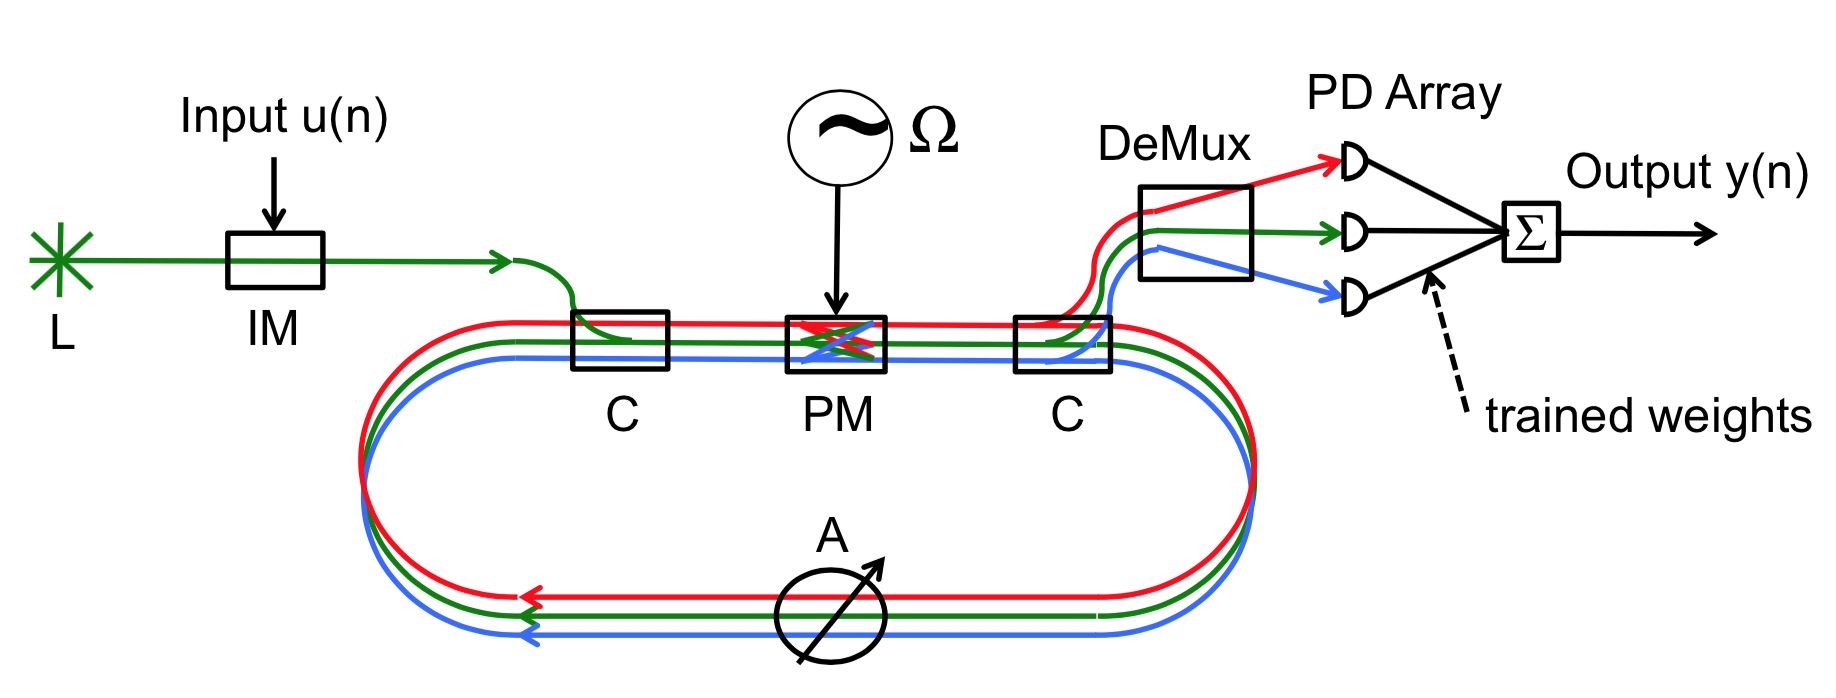
\includegraphics[width=.7\textwidth]{wdm_rc_principle.png}
		\caption{\cite{AkroutAkram2016Pprc}}
	\end{figure}
	\begin{itemize}
		\item \textbf{Wavelength Division Multiplexing} of the neurons
		\item Input: Monochromatic light source modulated in amplitude (data)
		\item The reservoir is the \textbf{ring cavity}
		\item Wavelength coupling handled by an intra-cavity \textbf{phase modulator}
		\item Output : wavelength demultiplexing and linear combination
	\end{itemize}
\end{frame}

\begin{frame}{Frequency coupling of the neurons}
	\begin{itemize}
		\item Transfer function of a phase modulator
		\begin{equation*}
			E e^{i\omega t} \overset{\Omega}{\longrightarrow} E e^{i\omega t} e^{i m \sin{(\Omega t)}} = E \sum_{n=-\infty}^{\infty} J_n(m) e^{i(\omega+n \Omega)t}
		\end{equation*}
		\item $J_n$ : Bessel function of order $n$
		\item $m$ : modulation depth ($m \leq 2$ experimentally)
		\item \textbf{Drawback : limited number of usable neurons} $\Longrightarrow$ \textbf{13 neurons}
	\end{itemize}
	\begin{columns}
		\begin{column}{.5\textwidth}
			\begin{figure}
				\centering
				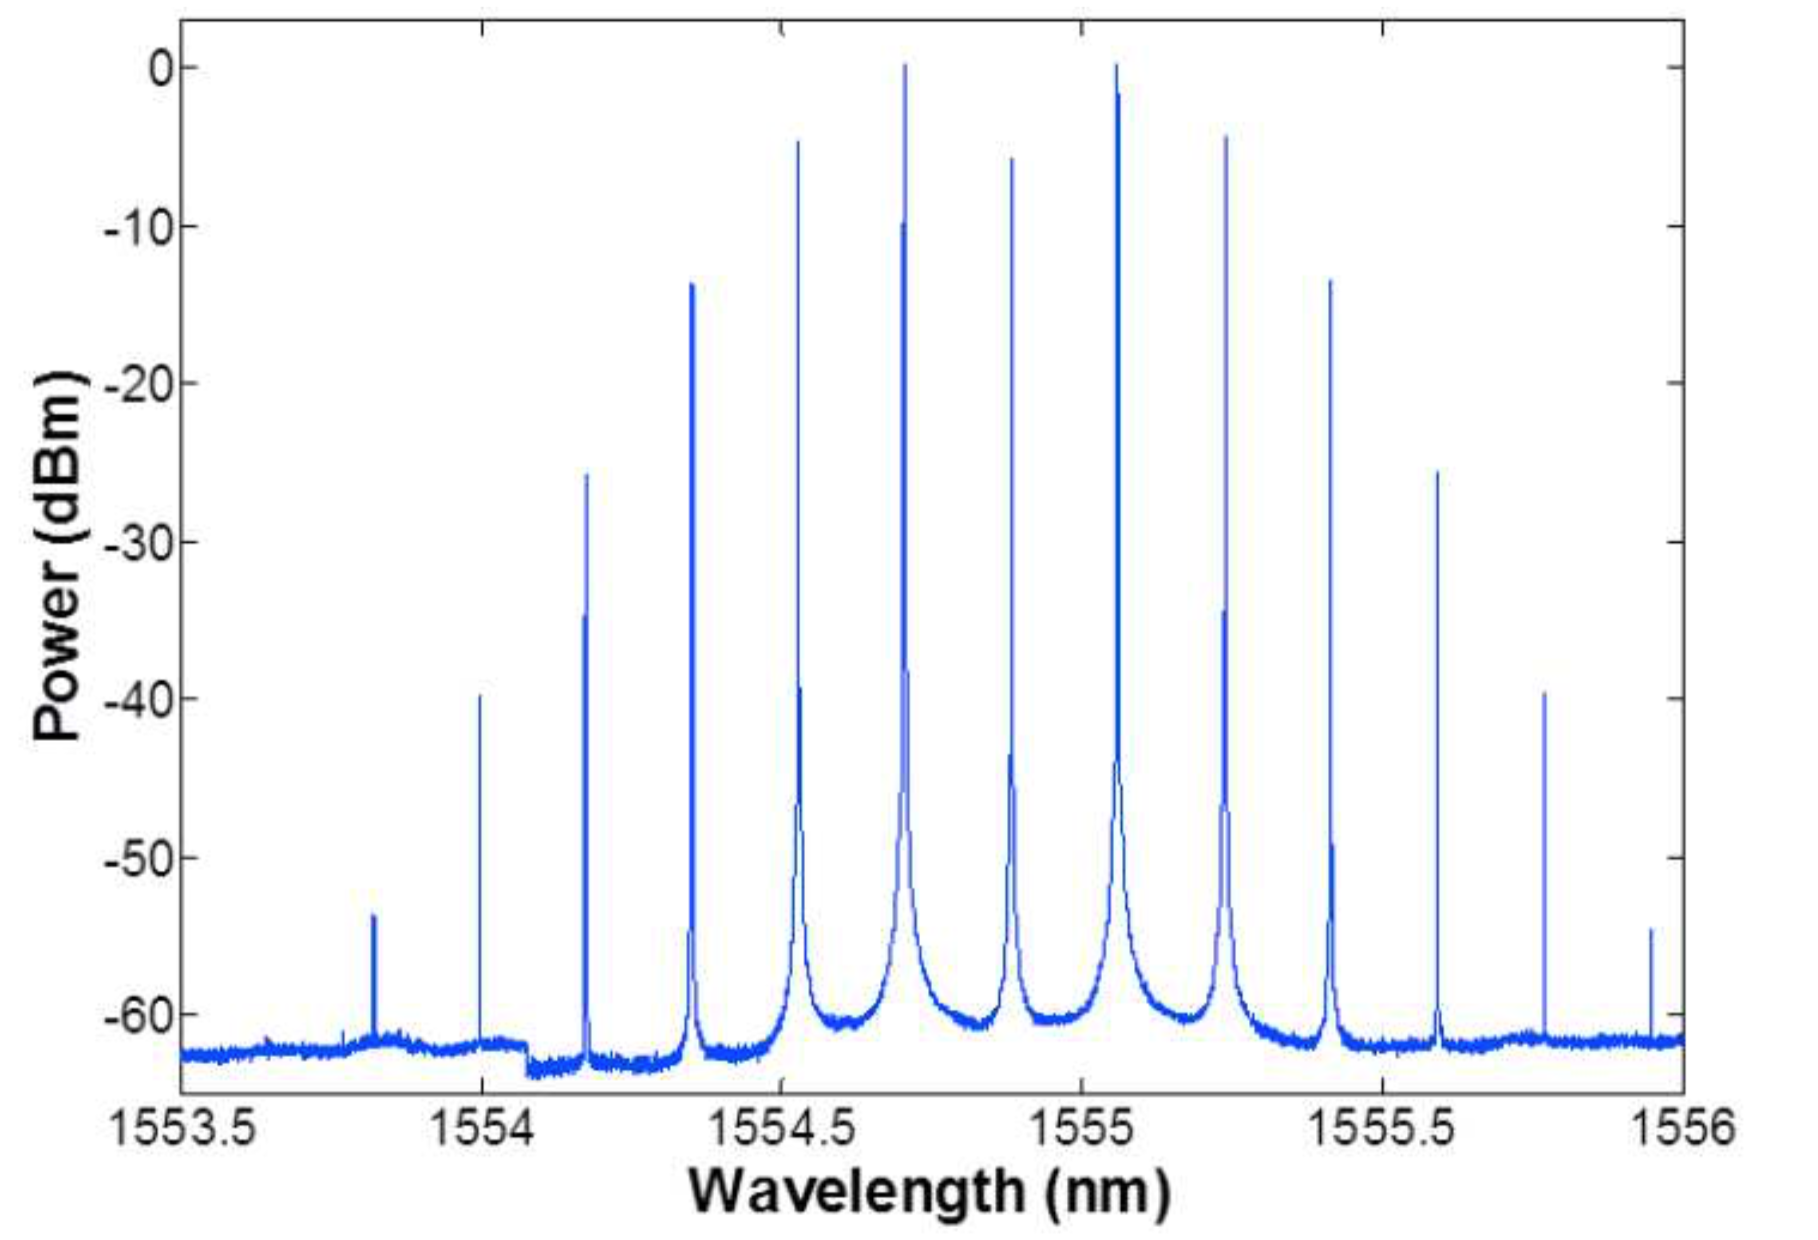
\includegraphics[width=\textwidth]{power-in-neurons.png}
			\end{figure}
		\end{column}%
		\begin{column}{.5\textwidth}
			\begin{figure}
				\centering
				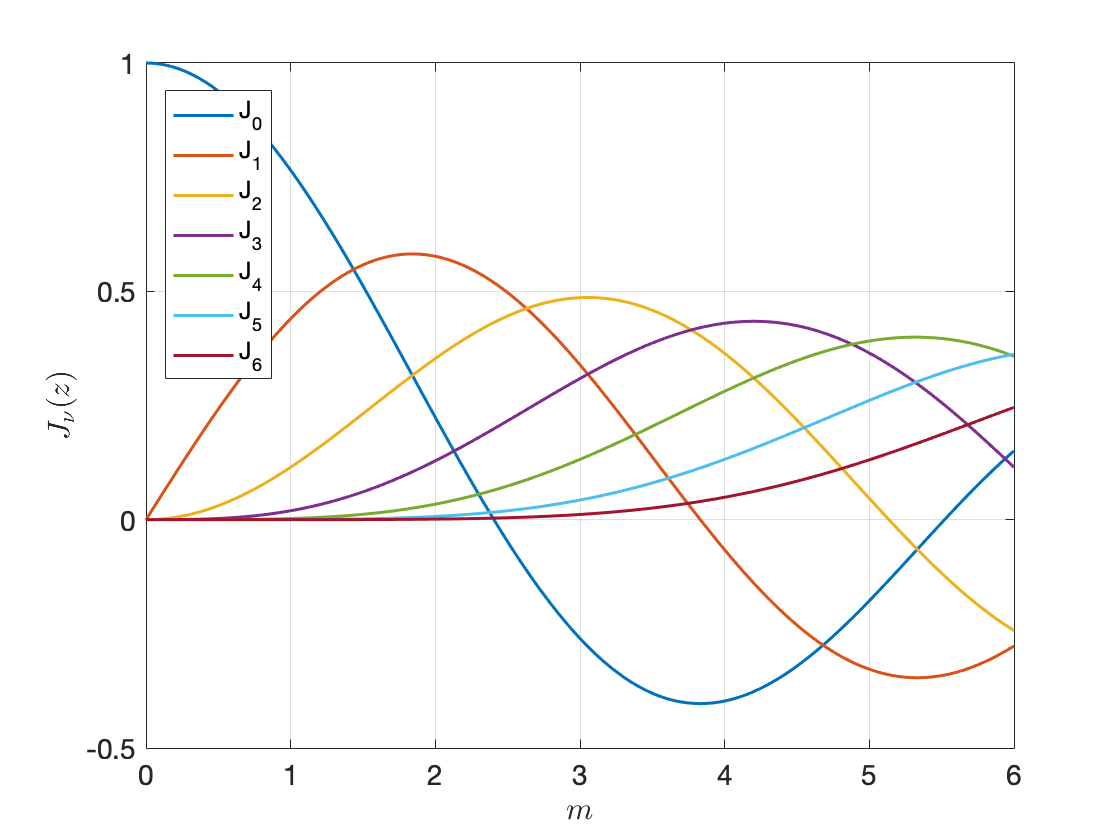
\includegraphics[width=\textwidth]{bessel.png}
			\end{figure}
		\end{column}
	\end{columns}
\end{frame}

\begin{frame}{Mathematical model}
	\begin{itemize}
		\item Neurons encoded in complex phaser representation of the electric field
		\item State vector :
		\begin{equation*}
			\mathbf{x} = \sum_{i=-\eta}^\eta x_i \hat{\mathbf{e}}_i
		\end{equation*}
		\item Basis vectors :
		\begin{equation*}
			\hat{\mathbf{e}}_n = e^{i\omega_n t} = e^{i (\omega+n \Omega)t}
		\end{equation*}
		\item Phase modulator frequency coupling transfer matrix :
		\begin{equation*}
			\mathbf{J} = \begin{bmatrix}
				J_0(m) & J_{-1}(m) & \dots & J_{-\eta}(m) & \dots & J_{-2\eta}(m) \\
				J_1(m) & J_0(m) & \dots & J_{-\eta+1}(m) & \dots & J_{-2\eta+1}(m) \\
				\vdots & \vdots &  & \vdots &  & \vdots \\
				J_{2\eta}(m) & J_{2\eta-1}(m) & \dots & J_\eta(m) & \dots & J_0(m)
			\end{bmatrix}
		\end{equation*}
	\end{itemize}
\end{frame}

\begin{frame}{Mathematical model}
	\begin{itemize}
		\item Acquired phase factor matrix :
		\begin{equation*}
			\Phi = \begin{bmatrix}
				e^{i\phi_{-\eta}} & 0 & \dots & 0 \\
				0 & e^{i\phi_{-\eta+1}} &  & 0 \\
				\vdots &  & \ddots & \\
				0 & 0 & \dots & e^{i\phi_{\eta}}
			\end{bmatrix}
		\end{equation*}
		\item $\alpha$ and $\beta$ : feedback and input gains		
	\end{itemize}
		\begin{alertblock}{Dynamics and output of the reservoir}
			\begin{align}
				\mathbf{x}(n+1) &= \alpha \Phi \mathbf{J} \bigg ( \mathbf{x}(n) + \beta u(n+1)~\hat{\mathbf{e}}_0 \bigg ) \nonumber \\
				y(n+1) &= \sum_{i=-\eta}^\eta W_i^{\text{out}} ~ |x_i(n)|^2 \nonumber
			\end{align}	
		\end{alertblock}
		\centering
		$\hookrightarrow$ Linear reservoir with quadratic output
\end{frame}













